\section{系统总体设计}

	系统总体结构组成如\Cref{overall_structure}所示,省略一段文字省略一段文字省略一段文字省略一段文字省略一段文字省略一段文字省略一段文字省略一段文字省略一段文字省略一段文字省略一段文字省略一段文字省略一段文字省
		
	\begin{figure}[H]
		\centering
		% 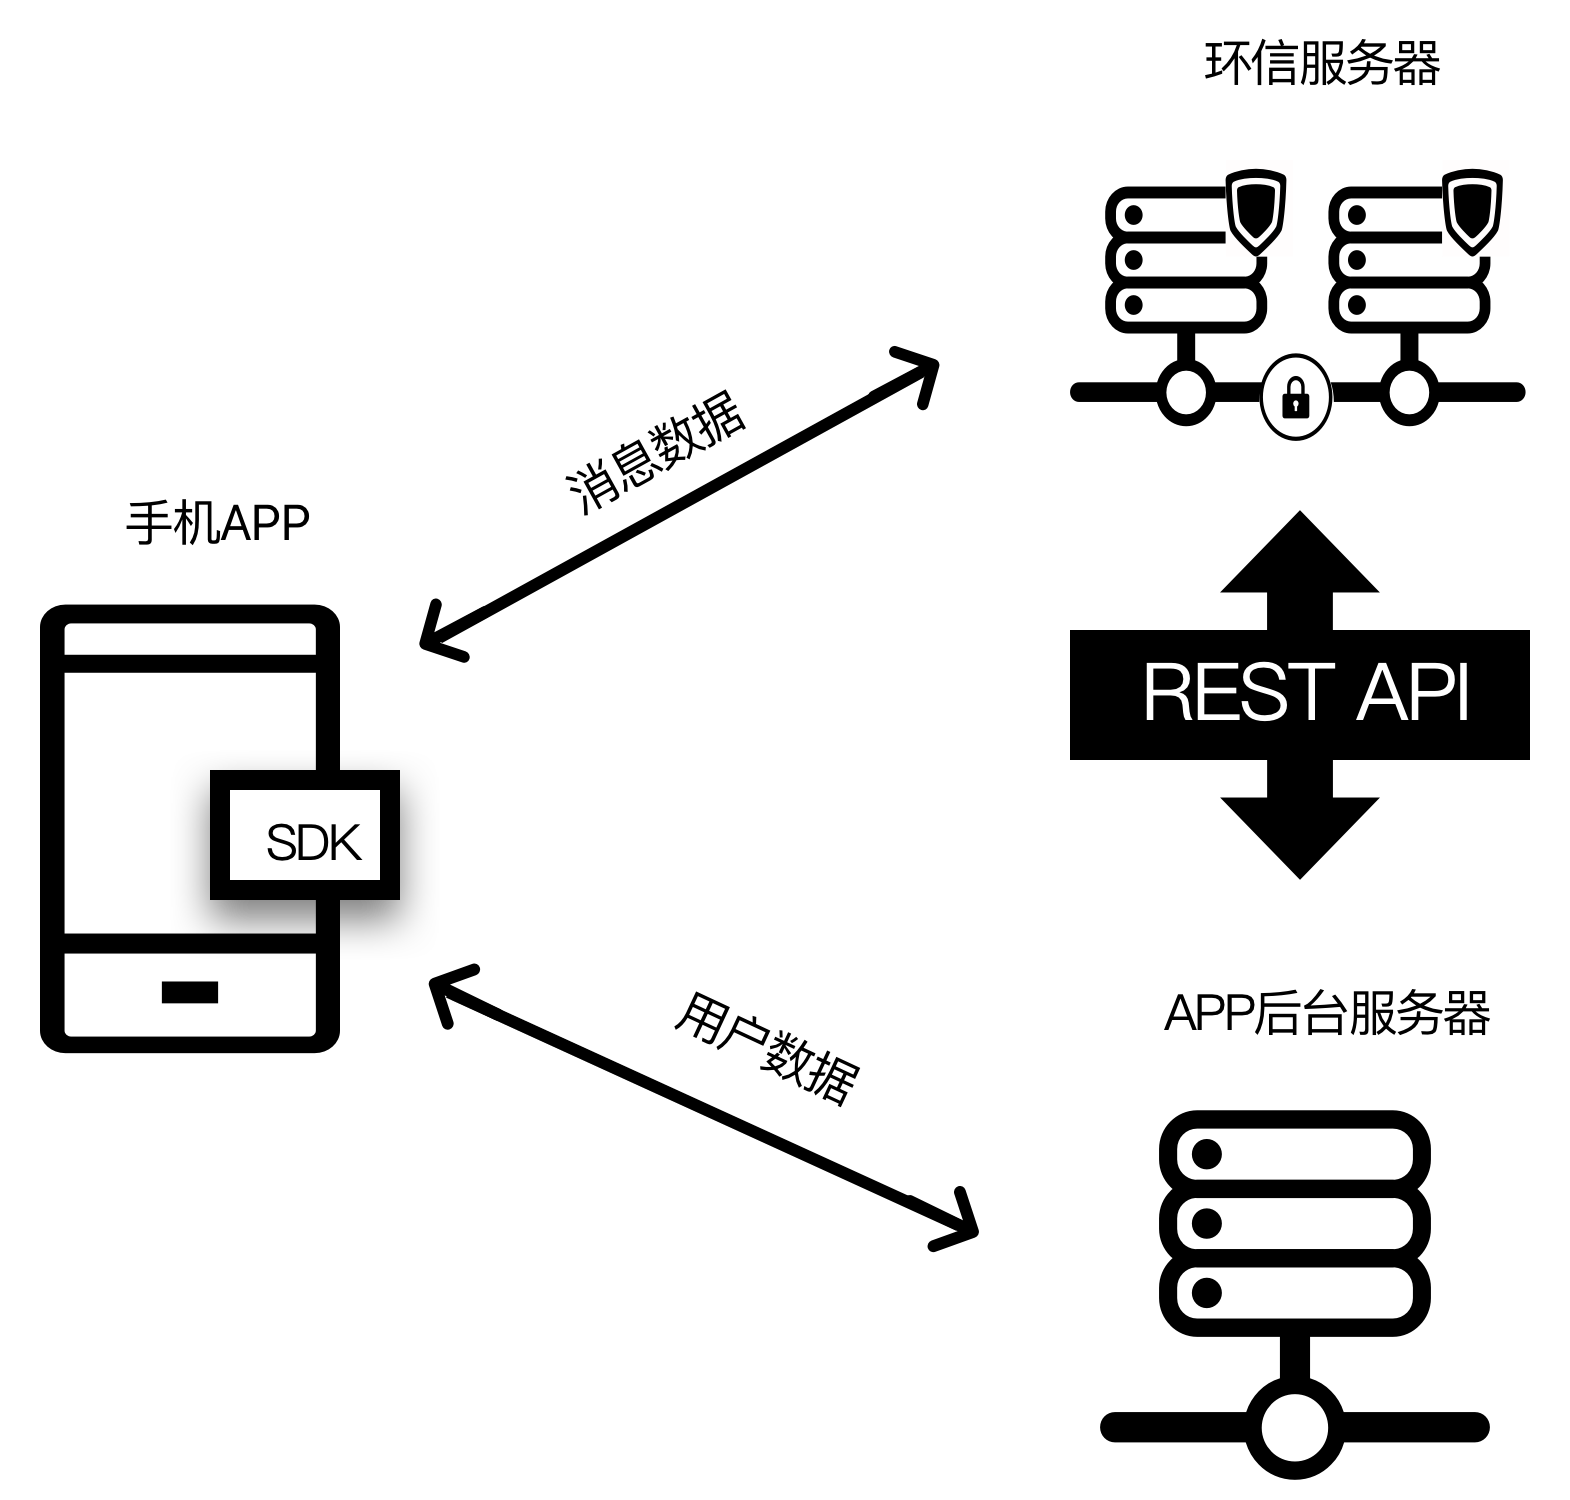
\includegraphics[width=0.80\textwidth]{images/all_design}
		\caption{系统总体结构组成}
		\label{overall_structure}
	\end{figure}
	
	\subsection{服务端总体设计}
	
		服务端的实现省略一段文字省略一段文字省略一段文字省略一段文字省略一段文字省略一段文字省略一段文字省略一段文字省略一段文字省略一段文字省略一段文字省略一段文字省略一段文字省		  
		  
		 省略一段文字省略一段文字省略一段文字省略一段文字省略一段文字省略一段文字省略一段文字省略一段文字省略一段文字省略一段文字省略一段文字省略一段文字省略一段文字省
		 
		  		  
		  
	\subsection{客户端总体设计}
		
		客户端采用分层的架构进行设计,上层实现依赖于下层设计\scite{cite_分层设计},自下而上分为基础层、数据层、组件层、表现层、应用层,整体设计结构如\Cref{mobile_overall_design}所示。
	
	\begin{figure}[H]
		\centering
		% 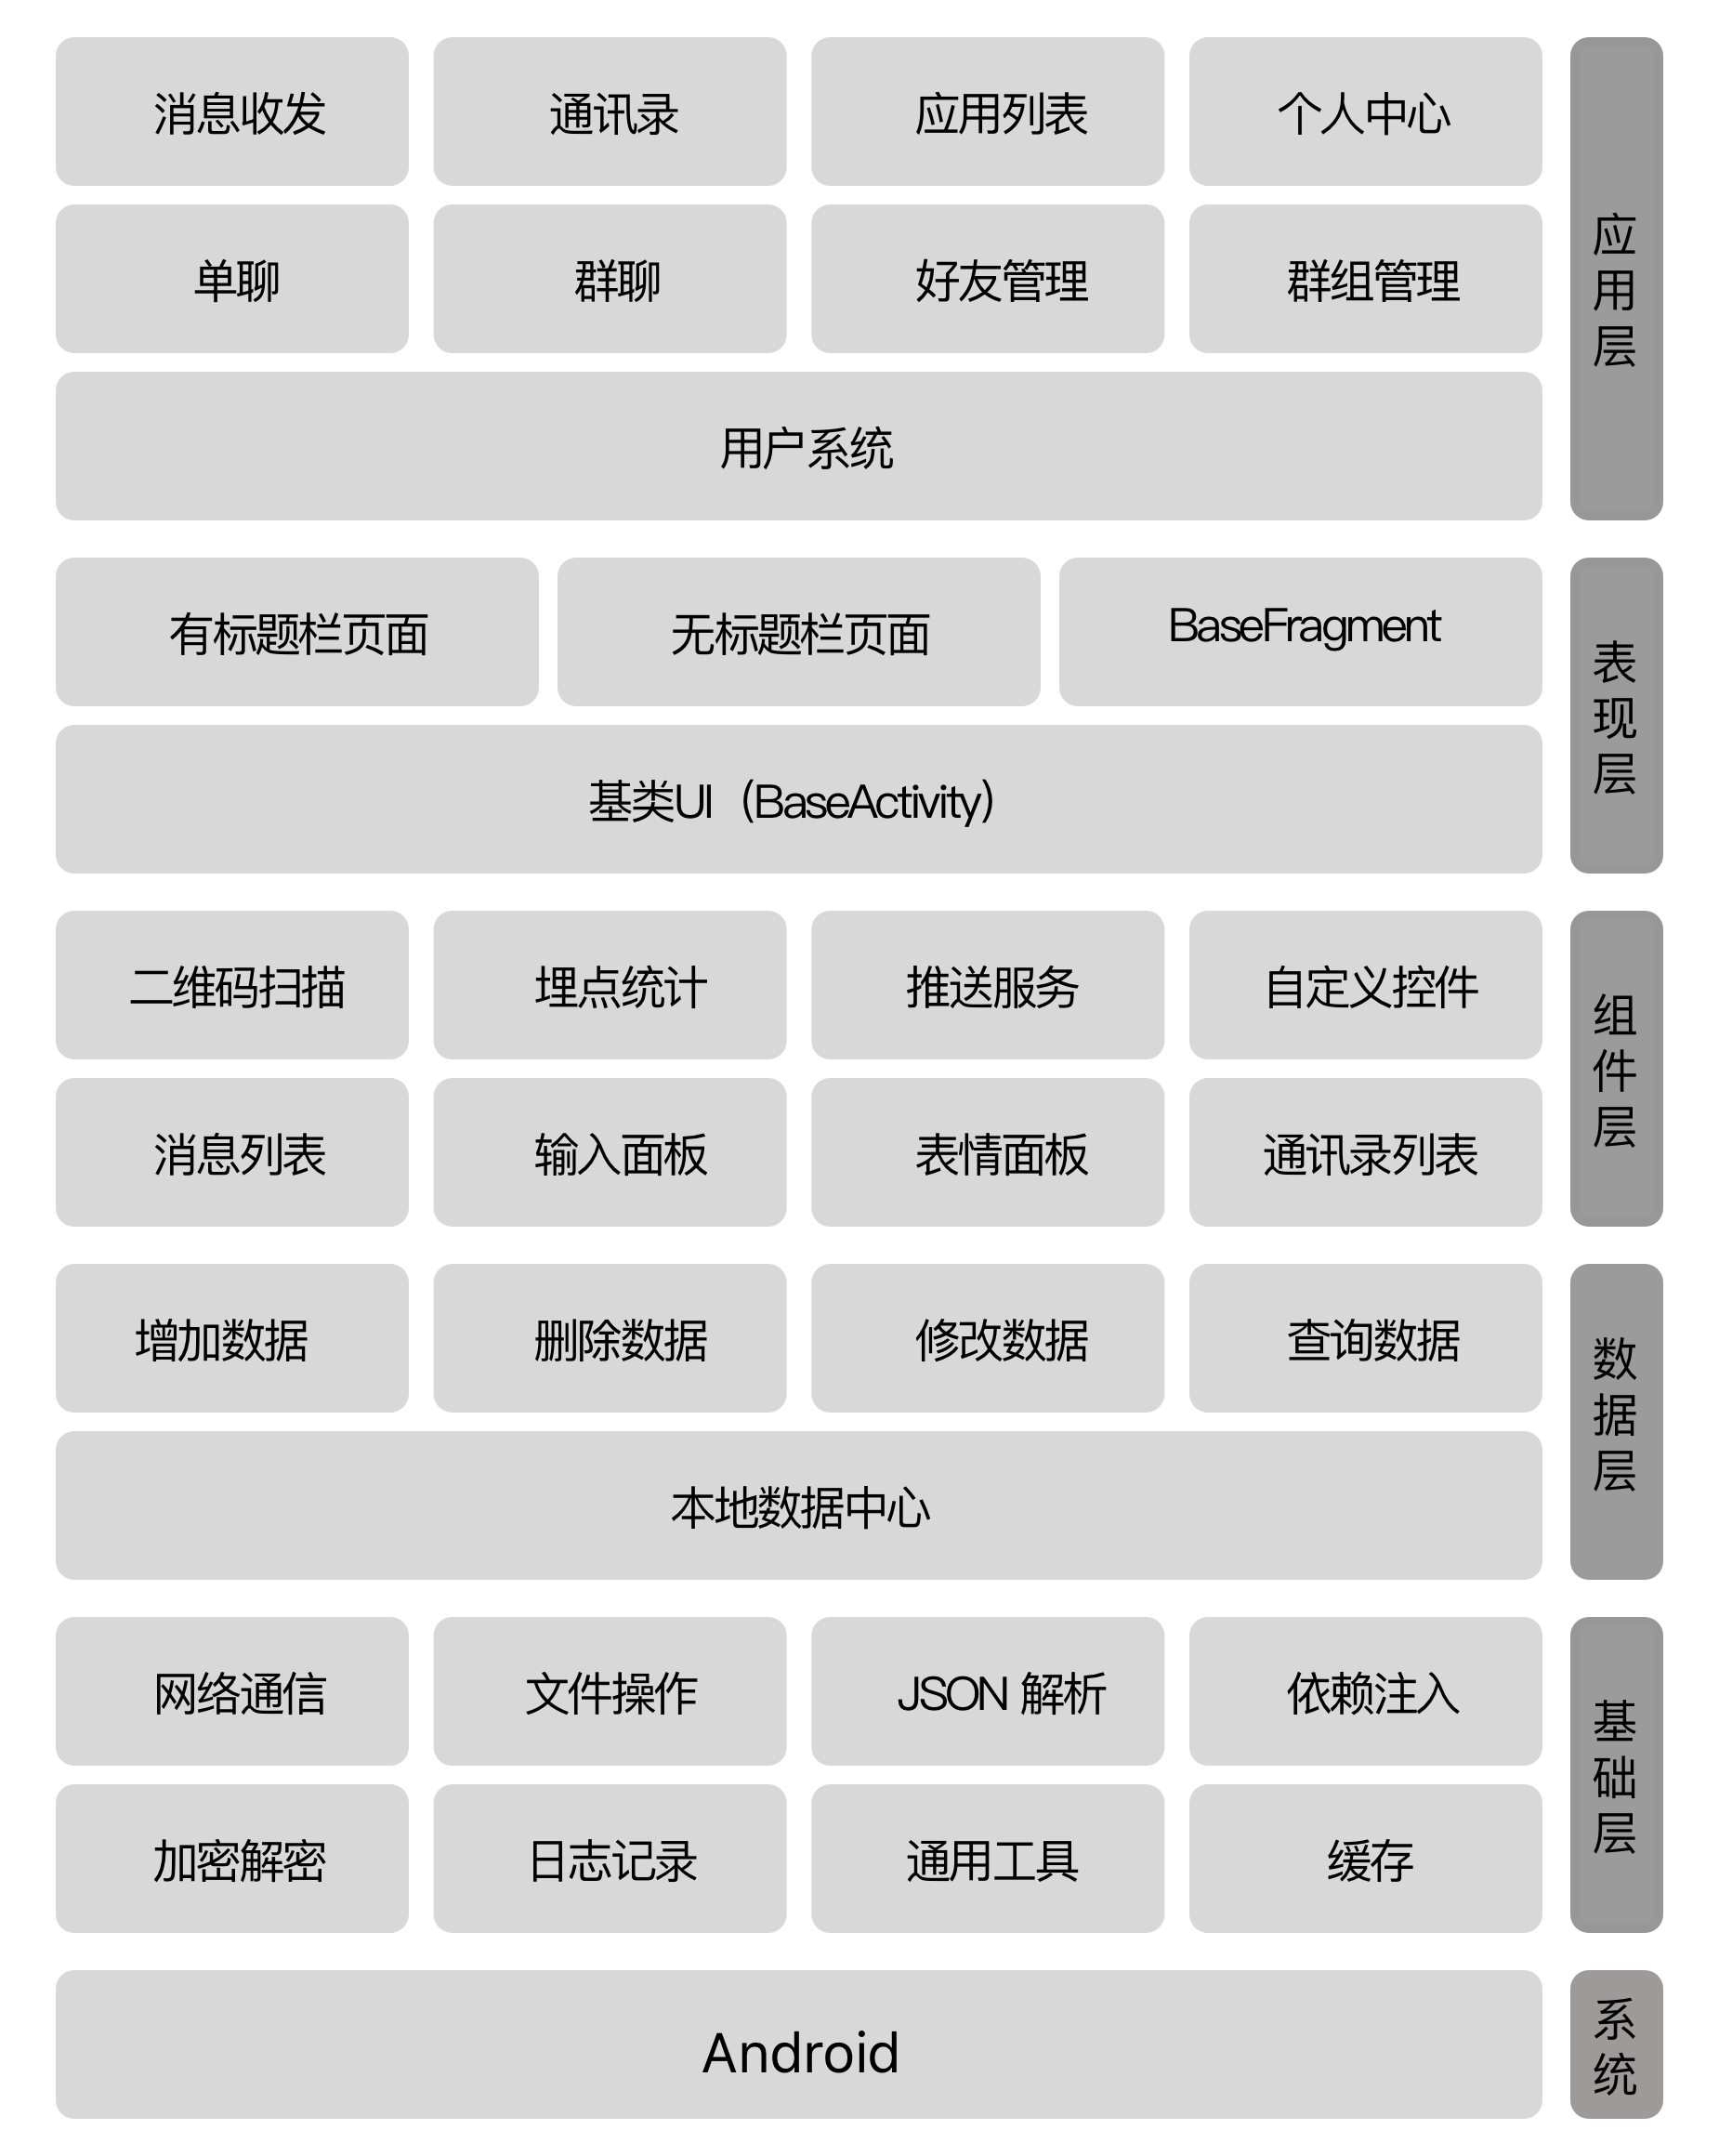
\includegraphics[width=0.95\textwidth]{images/mobile_design}
		\caption{移动端总体设计结构}
		\label{mobile_overall_design}
	\end{figure}


	\begin{enumerate}[fullwidth,itemindent=2em,listparindent=2em]
	
		\item 设计概述
		
		省略一段文字省略一段文字省略一段文字省略一段文字省略一段文字省略一段文字省略一段文字省略一段文字省略一段文字省略一段文字省略一段文字省略一段文字省略一段文字省
		
		省略一段文字省略一段文字省略一段文字省略一段文字省略一段文字省略一段文字省略一段文字省略一段文字省略一段文字省略一段文字省略一段文字省略一段文字省略一段文字省
		
		\item 设计概述
		
		省略一段文字省略一段文字省略一段文字省略一段文字省略一段文字省略一段文字省略一段文字省略一段文字省略一段文字省略一段文字省略一段文字省略一段文字省略一段文字省
		
		省略一段文字省略一段文字省略一段文字省略一段文字省略一段文字省略一段文字省略一段文字省略一段文字省略一段文字省略一段文字省略一段文字省略一段文字省略一段文字省

		\item 设计概述
		
		省略一段文字省略一段文字省略一段文字省略一段文字省略一段文字省略一段文字省略一段文字省略一段文字省略一段文字省略一段文字省略一段文字省略一段文字省略一段文字省
		
		省略一段文字省略一段文字省略一段文字省略一段文字省略一段文字省略一段文字省略一段文字省略一段文字省略一段文字省略一段文字省略一段文字省略一段文字省略一段文字省

			
		

	\end{enumerate}

	\subsection{数据库总体设计}

		
		省略一段文字省略一段文字省略一段文字省略一段文字省略一段文字省略一段文字省略一段文字省略一段文字省略一段文字省略一段文字省略一段文字省,表格使用,表格使用,表格使用,表格使用,表格使用,表格使用,如\Cref{tab:db_table_user}所示。
	
		\begin{table}[H]
		\centering
		\caption{User 用户表}
		\zihao{5}
		\label{tab:db_table_user}
		\begin{tabular}{p{0.21\textwidth}p{0.21\textwidth}p{0.21\textwidth}p{0.21\textwidth}}
		\hline
		字段          & 数据类型         & 字段含义   & 约束条件     \\ \hline
		id          & INT(11)      & 用户ID & 主键、非空、自增 \\
		im\_id      & VARCHAR(256) & 环信ID & 唯一       \\ 
		account     & VARCHAR(45)  & 用户名  & 唯一       \\ 
		nick\_name  & VARCHAR(100) & 昵称   & 无        \\
		password    & VARCHAR(256) & 密码   & 非空       \\ 
		email       & VARCHAR(45)  & 邮箱   & 无        \\
		mobile      & VARCHAR(45)  & 手机号  & 唯一        \\ 
		sex         & INT(11)      & 性别   & 无        \\ 
		signature   & VARCHAR(512) & 签名   & 无        \\
		avatar      & VARCHAR(256) & 头像   & 无        \\
		is\_deleted & TINYINT(4)   & 删除标志 & 无        \\ \hline
		\end{tabular}
		\end{table}
		
 \clearpage